\documentclass[a4paper]{article} 

\input{head}

\usepackage{float}
\usepackage[T1]{fontenc}
\usepackage{hyperref}
\usepackage{subcaption}

\begin{document}

\fancyhead[C]{}
\hrule \medskip
\begin{minipage}{0.295\textwidth} 
  \raggedright
  \scriptsize
  Michele Scomina \hfill\\   
  IN2000214\hfill\\
  mscomina@gmail.com\hfill\\
  michele.scomina@studenti.units.it
\end{minipage}
\begin{minipage}{0.4\textwidth} 
\centering 
\large 
\textbf{OSU Benchmarks - Broadcast and Reduce}\\ 
\end{minipage}
\begin{minipage}{0.295\textwidth} 
\raggedleft
\today\hfill\\
\end{minipage}
\medskip\hrule 
\bigskip

\setlength{\parskip}{4pt}

\begin{abstract}
This is the report for Exercise 1. In this report we showcase the steps taken to compile the OSU Benchmark and run said benchmarks on two collective operations on the ORFEO cluster, as described in the \href{https://github.com/Foundations-of-HPC/High-Performance-Computing-2023/blob/main/ASSIGNMENTS/exercise1/exercise1.md}{GitHub repository}.
\end{abstract}

\section{OSU Benchmarks}

The OSU Micro-Benchmarks (OMB) are a collection of benchmarks designed to measure the performance of communication operations in MPI. They provide a standardized way to evaluate metrics such as latency and bandwidth for different message sizes and numbers of processes.

For this exercise, two collective communication operations are considered: \texttt{MPI\_Bcast} and \texttt{MPI\_Reduce}. The corresponding OSU benchmarks are run on the ORFEO cluster under different configurations to evaluate their communication performance.

\subsection{MPI\_Bcast}

\texttt{MPI\_Bcast} is a collective operation that broadcasts a message from a designated root process to all other processes in the communicator. The data provided by the root is therefore replicated across all processes.

The OSU broadcast benchmark measures the time required to perform this operation for different message sizes and numbers of processes. This allows us to evaluate how the broadcast performance changes as the amount of data and the number of participating processes increase.

\begin{figure}[H]
    \centering
    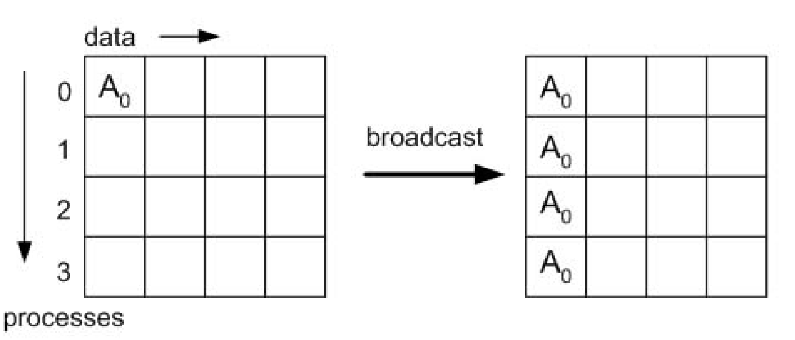
\includegraphics[width=0.7\textwidth]{MPI_BCast_graphical.png}
    \caption{Graphical representation of \texttt{MPI\_BCast}.}
    \label{fig:mpi_bcast_graphical}
\end{figure}

\subsection{MPI\_Reduce}

\texttt{MPI\_Reduce} is a collective operation that combines data from all processes using a specified reduction operation, such as a sum, and stores the resulting value on a designated root process.

The OSU reduce benchmark measures the time required to perform this operation for different message sizes and numbers of processes. This allows us to evaluate the communication and reduction overhead as the number of processes and the amount of data increase.

\begin{figure}[H]
    \centering
    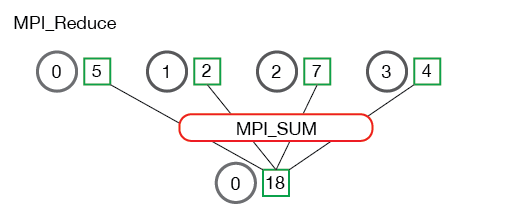
\includegraphics[width=0.5\textwidth]{MPI_Reduce_graphical.png}
    \caption{Graphical representation of \texttt{MPI\_Reduce}.}
    \label{fig:mpi_reduce_graphical}
\end{figure}

\section{Compiling}

The OSU Micro-Benchmarks are compiled directly on the ORFEO cluster using the MPI implementation that will also be used to run the benchmarks. This ensures that the generated binaries are compatible with the cluster environment and the selected MPI implementation.

The compilation is performed through a Slurm job on the \texttt{THIN} partition. The appropriate MPI module is loaded before compiling, after which the OSU Micro-Benchmarks source code is downloaded and configured using the MPI compiler wrappers \texttt{mpicc} and \texttt{mpicxx}:

\begin{verbatim}
./configure CC=mpicc CXX=mpicxx --prefix="${OSU_PATH}"
make
make install
\end{verbatim}

The resulting binaries are installed in a custom directory specified by \texttt{OSU\_PATH}, allowing them to be used when running the benchmarks without recompiling them for each experiment. Separating the compilation step from the benchmark runs also avoids unnecessarily using compute resources for compilation. Scripts are provided in the repository for ease of use.

\section{Benchmark results}

The benchmarks were executed on the ORFEO cluster using different numbers of MPI processes and different collective communication algorithms. The three algorithms considered for each collective operation are:

\begin{itemize}
\item \texttt{MPI\_Bcast}:
\begin{itemize}
\item \textbf{Basic linear:} the root process sends the message directly to each process sequentially.
\item \textbf{Pipeline:} the message is divided into segments that are forwarded between processes, allowing communication to overlap.
\item \textbf{Binomial tree:} processes are organized in a tree structure, allowing the message to reach all processes in approximately $\log_2(P)$ communication steps.
\end{itemize}

\item \texttt{MPI\_Reduce}:
\begin{itemize}
    \item \textbf{Linear:} processes send their data directly towards the root, which performs the reduction.
    \item \textbf{Pipeline:} data is divided into segments and reduction is performed progressively as segments move through the processes.
    \item \textbf{In-order binary:} processes are organized as a binary tree, with partial results combined at each level before reaching the root.
\end{itemize}


\end{itemize}

For each configuration, the benchmark was executed 10 times and the measured results were collected for different message sizes. The number of MPI processes was varied from 2 to the maximum number supported by the allocated nodes, in steps of two processes.

\newpage

\subsection{Point-to-Point latency}

\begin{figure}[H]
\centering
\includegraphics[width=0.75\textwidth]{naive_model.pdf}
\caption{Point-to-point latency measured with two MPI processes.}
\label{fig:latency}
\end{figure}

The point-to-point latency provides a baseline for comparison with the collective communication results. As expected, the latency remains approximately constant for small messages, up to around 128 bytes, before increasing progressively with message size. In the log-log plot, this produces the characteristic curved shape visible in Figure~\ref{fig:latency}. The latency is approximately $1\mu\mathrm{s}$ for the smallest messages and increases to $400\mu\mathrm{s}$ as the message size approaches the maximum tested value of 4 MB.


\subsection{MPI\_Bcast}

\begin{figure}[H]
    \centering

    \begin{subfigure}[b]{0.48\textwidth}
        \centering
        \includegraphics[width=\textwidth]{osu_bcast.pdf}
        \caption{\texttt{MPI\_BCast} latency measured across different MPI processes amounts and collective algorithms.}
        \label{fig:osu_bcast_standard}
    \end{subfigure}
    \hfill
    \begin{subfigure}[b]{0.48\textwidth}
        \centering
        \includegraphics[width=\textwidth]{osu_bcast_fixed.pdf}
        \caption{\texttt{MPI\_BCast} latency across different packet sizes.}
        \label{fig:osu_bcast_fixed}
    \end{subfigure}

    \caption{Plots for \texttt{MPI\_BCast}.}
    \label{fig:mpi_bcast_scaling}
\end{figure}

The results for \texttt{MPI\_Bcast} show clear differences in how the three collective algorithms scale with the number of processes and the message size. The basic linear algorithm exhibits the expected linear increase in latency as the number of processes grows. The pipeline algorithm follows a similar trend for small messages, but its performance improves considerably for larger messages and higher numbers of processes. The binomial tree algorithm scales better with the number of processes overall, although for large messages and a high number of processes, the pipeline algorithm achieves slightly lower latency.

The fixed-message-size plots provide a more detailed comparison between the algorithms. For the smallest message size, 512 bytes, all three algorithms exhibit a similar scaling shape as the number of processes increases, although they operate at slightly different latency levels. In this case, the binomial tree algorithm has the lowest latency, followed by the basic linear algorithm, while the pipeline algorithm performs slightly worse. As the message size increases to 64~KB and 1~MB, the relative performance changes: the pipeline algorithm becomes increasingly advantageous as throughput becomes more important, eventually achieving the lowest latency for large messages and high process counts. The binomial tree algorithm maintains good scaling and remains competitive, while the basic linear algorithm becomes increasingly affected by the growing number of processes.

\subsection{MPI\_Reduce}

\begin{figure}[H]
    \centering

    \begin{subfigure}[b]{0.48\textwidth}
        \centering
        \includegraphics[width=\textwidth]{osu_reduce.pdf}
        \caption{\texttt{MPI\_Reduce} latency measured across different MPI processes amounts and collective algorithms.}
        \label{fig:osu_reduce_standard}
    \end{subfigure}
    \hfill
    \begin{subfigure}[b]{0.48\textwidth}
        \centering
        \includegraphics[width=\textwidth]{osu_reduce_fixed.pdf}
        \caption{\texttt{MPI\_Reduce} latency across different packet sizes.}
        \label{fig:osu_reduce_fixed}
    \end{subfigure}

    \caption{Plots for \texttt{MPI\_Reduce}.}
    \label{fig:mpi_reduce_scaling}
\end{figure}

The \texttt{MPI\_Reduce} results show a different performance trade-off between the three algorithms. The linear algorithm achieves the lowest latency for small messages and is particularly effective at 512 bytes. However, its latency increases significantly as the message size and number of processes grow, resulting in poor scaling for larger messages combined with high process counts.

The pipeline algorithm has the highest latency for small messages and its latency increases considerably with the number of processes. However, its performance improves relative to the other algorithms as the message size increases. For large messages, the pipeline becomes the most efficient algorithm for smaller numbers of processes, benefiting from the ability to overlap communication and reduction across message segments.

The in-order binary algorithm provides more consistent scaling across the tested configurations. Its tree-based structure limits the increase in communication steps as the number of processes grows, making it competitive across different message sizes. For large numbers of processes, it generally achieves the lowest latency, while for very small messages the linear algorithm remains more efficient.

\subsection{Normalized Latency}

\begin{figure}[H]
    \centering
    \includegraphics[width=0.75\textwidth]{normalized_latency.pdf}
    \caption{Normalized latency for \texttt{MPI\_Bcast} and \texttt{MPI\_Reduce}.}
    \label{fig:normalized_latency}
\end{figure}

The normalized latency highlights how the communication cost scales with the number of processes relative to the message size. Since the benchmarks were executed on two nodes with 24 processes per node, configurations with up to 24 processes can be accommodated on a single node, while configurations with more than 24 processes require both nodes.

For \texttt{MPI\_Bcast}, the basic linear algorithm shows an approximately linear increase in normalized latency, with a noticeable increase around 24 processes. It grows from approximately $1\mu\mathrm{s}/B$ to $18\mu\mathrm{s}/B$. The pipeline algorithm scales more slowly and does not exhibit the same increase at 24 processes, reaching approximately $10\mu\mathrm{s}/B$. The binomial tree algorithm shows a more irregular behavior, with several smaller fluctuations, but follows an overall trend similar to the pipeline algorithm and reaches a comparable value.

For \texttt{MPI\_Reduce}, the linear algorithm again shows an approximately linear increase, with a steeper growth after 24 processes, reaching approximately $15\mu\mathrm{s}/B$. The pipeline algorithm follows a similar trend up to 24 processes, where a pronounced increase is observed, after which the normalized latency remains relatively stable at approximately $6\mu\mathrm{s}/B$. The in-order binary algorithm exhibits the most stable behavior, remaining close to $1\mu\mathrm{s}/B$ across the tested process counts.

\end{document}